% Homework template for Information Theory and Statistical Learning
% by Xiangxiang Xu <xiangxiangxu.thu@gmail.com>
% LAST UPDATE: Oct 3, 2019
\documentclass[a4paper]{article}
\usepackage[T1]{fontenc}
\usepackage{amsmath, amssymb, amsthm}
% amsmath: equation*, amssymb: mathbb, amsthm: proof
\usepackage{moreenum}
\usepackage{mathtools}
\usepackage{url}
\usepackage{enumitem}
\usepackage{bm}
\usepackage{graphicx}
\usepackage{subcaption}
\usepackage{booktabs} % toprule
\usepackage[mathcal]{eucal}
\usepackage{dsfont}
\usepackage[numbered,framed]{matlab-prettifier}
%% Definitions for Information Theory & Statistical Learning
%% UPDATED: Sep 30, 2019 by Xiangxiang 
\newcommand{\theterm}{Fall 2020}

\newcommand{\thecoursenameshort}{\textsc{Information Theory and Statistical Learning}}
\newcommand{\thecoursename}{
Tsinghua-Berkeley Shenzhen Institute\\
%\vspace*{0.1in}
\thecoursenameshort
}

\newcommand{\courseheader}{
\vspace*{-1in}
\begin{center}
\thecoursename \\
\theterm
\vspace*{0.1in}
\hrule
\end{center}
}
\newcommand{\uc}{\underline{c}}    % c, vec
\newcommand{\uv}{\underline{v}}    % x, vec
\newcommand{\uw}{\underline{w}}    % w, vec
\newcommand{\ux}{\underline{x}}    % x, vec
\newcommand{\uy}{\underline{y}}    % y, vec
\newcommand{\uz}{\underline{z}}    % z, vec
\newcommand{\um}{\underline{m}}    % m, vec
\newcommand{\ut}{\underline{t}}    % t, vec

\newcommand{\bA}{\mathbf{A}}    % A, mat
\newcommand{\bI}{\mathbf{I}}    % A, mat
\newcommand{\bN}{\mathbf{N}}    % n, mat
\newcommand{\bT}{\mathbf{T}}    % T, mat
\newcommand{\bU}{\mathbf{U}}    % U, mat
\newcommand{\bV}{\mathbf{V}}    % V, mat
\newcommand{\bQ}{\mathbf{Q}}    % Q, mat
\newcommand{\bX}{\mathbf{X}}    % X, mat

\newcommand{\bc}{\bm{c}}    % c, vec
\newcommand{\be}{\bm{e}}    % e, vec
\newcommand{\bu}{\bm{u}}    % u, vec
\newcommand{\bv}{\bm{v}}    % v, vec
\newcommand{\bw}{\bm{w}}    % w, vec
\newcommand{\bt}{\bm{t}}    % t, vec
\newcommand{\bx}{\bm{x}}    % x, vec
\newcommand{\by}{\bm{y}}    % y, vec
\newcommand{\bz}{\bm{z}}    % z, vec

\newcommand{\phib}{\bm{\phi}}    % phi, vec
\newcommand{\psib}{\bm{\psi}}    % psi, vec
\newcommand{\dtm}{\mathbf{B}}    %
\newcommand{\dtmt}{\tilde{\dtm}}    %
\newcommand{\Ab}{\mathbf{A}}    % A mat
\newcommand{\Kb}{\mathbf{K}}    % K mat
\newcommand{\Ib}{\mathbf{I}}    % I mat



\newcommand{\rvby}{\bm{\mathsf{y}}}    % y, rv. vec
\newcommand{\rvbx}{\bm{\mathsf{x}}}    % x, rv. vec
% \newcommand{\bm}{\bm{m}}    % m, vec
\newcommand{\bzero}{\bm{0}}    % 0, vec

\newcommand{\balpha}{\bm{\alpha}}    % alpha, vec
\newcommand{\bphi}{\bm{\phi}}    % phi, vec
\newcommand{\bpsi}{\bm{\psi}}    % psi, vec
\newcommand{\bxi}{\bm{\xi}}    % xi, vec
\newcommand{\btheta}{\bm{\theta}}    % theta, vec
\newcommand{\bmu}{\bm{\mu}}    % mu, vec

\newcommand{\bLambda}{\bm{\Lambda}}    % Sigma, mat
\newcommand{\bSigma}{\bm{\Sigma}}    % Sigma, mat

\newcommand{\cF}{\mathcal{F}}  
\newcommand{\cL}{\mathcal{L}}  
\newcommand{\cX}{\mathcal{X}}  
\newcommand{\cY}{\mathcal{Y}}  

\newcommand{\rvx}{\mathsf{x}}    % x, r.v.
\newcommand{\rvy}{\mathsf{y}}    % y, r.v.
\newcommand{\rvz}{\mathsf{z}}    % z, r.v.
\newcommand{\rvw}{\mathsf{w}}    % w, r.v.
\newcommand{\rvv}{\mathsf{v}}    % v, r.v.
\newcommand{\rvm}{\mathsf{m}}    % m, r.v.
\newcommand{\rvt}{\mathsf{t}}    % t, r.v.
\newcommand{\rvH}{\mathsf{H}}    % H, r.v.
\newcommand{\urvx}{\underline{\mathsf{x}}}    % x, r.v. vec
\newcommand{\urvy}{\underline{\mathsf{y}}}    % y, r.v. vec
\newcommand{\urvz}{\underline{\mathsf{z}}}    % z, r.v. vec
\newcommand{\urvw}{\underline{\mathsf{w}}}    % w, r.v. vec
\newcommand{\urvt}{\underline{\mathsf{t}}}    % t, r.v. vec


\newcommand{\defeq}{\triangleq} %\coloneqq
\newcommand{\reals}{\mathbb{R}}
\newcommand{\T}{\mathrm{T}}    % transpose
\newcommand{\F}{\mathrm{F}}    % Frobenius
\newcommand{\BLS}{\mathrm{BLS}}    % BLS
\newcommand{\LLS}{\mathrm{LLS}}    % LLS
\newcommand{\MVU}{\mathrm{MVU}}    % MVU
\newcommand{\dd}{\mathrm{d}}  

\DeclareMathOperator*{\maximize}{maximize}    % maximize
\DeclareMathOperator*{\minimize}{minimize}    % minimize
\newcommand{\st}{\mathrm{subject~to}}    % minimize

% \newcommand{\E}[1]{\mathbb{E}\left[{#1}\right]}
% \newcommand{\Prob}[1]{\mathbb{P}\left({#1}\right)}
\DeclareMathOperator*{\argmax}{arg\,max}
\DeclareMathOperator*{\argmin}{arg\,min}
\DeclareMathOperator*{\argsup}{arg\,sup}
\DeclareMathOperator*{\arginf}{arg\,inf}
\DeclareMathOperator{\diag}{diag}
\DeclareMathOperator{\tr}{tr}
\DeclareMathOperator{\Cov}{Cov}
\DeclareMathOperator{\var}{var}
\DeclareMathOperator{\cov}{cov}
\DeclareMathOperator{\MSE}{MSE}
\DeclareMathOperator{\1}{\mathds{1}} % dsfont required
\DeclareMathOperator{\E}{\mathbb{E}}
\DeclareMathOperator{\Prob}{\mathbb{P}}
\DeclareMathOperator{\im}{im}
\DeclareMathOperator{\rank}{rank}
\DeclareMathOperator{\Bern}{Bern}
\DeclareMathOperator{\Binom}{Binom}

\newcommand\independent{\protect\mathpalette{\protect\independenT}{\perp}}
\def\independenT#1#2{\mathrel{\rlap{$#1#2$}\mkern2mu{#1#2}}}

%%% Local Variables:
%%% mode: latex
%%% TeX-master: "ithw"
%%% End:


\lstset{
  style              = Matlab-editor,
  captionpos         =b,
  basicstyle         = \mlttfamily,
  escapechar         = ",
  mlshowsectionrules = true,
}
\begin{document}
\courseheader



\newcounter{hwcnt}
\setcounter{hwcnt}{1} % set to the times of Homework

\begin{center}
  \underline{\bf Homework \thehwcnt} \\
\end{center}
\begin{flushleft}
  \textcolor{gray}{HANMO CHEN}\hfill
  \today
\end{flushleft}
\hrule

\vspace{2em}
\setlist[enumerate,1]{label=\thehwcnt.\arabic*.}
\setlist[enumerate,2]{label=(\alph*)}
\setlist[enumerate,3]{label=\roman*.}
\setlist[enumerate,4]{label=\greek*)}


\newcommand{\EX}{\mathbb{E}}

\flushleft
\rule{\textwidth}{1pt}
\begin{itemize}
\item {\bf Acknowledgments: \/} 
  \textcolor{gray}{For Problem 1.2(b), I refer to some answer on StackExchange \small{\url{https://math.stackexchange.com/a/108303}}}
  % \textcolor{gray}{This template takes some materials from course CSE 547/Stat 548 of Washington University: \small{\url{https://courses.cs.washington.edu/courses/cse547/17sp/index.html}}.}

  % \textcolor{red}{If you refer to other materials in your homework, please list here.}
\item {\bf Collaborators: \/}
  \textcolor{gray}{I finish this homework all by myself.} 
% \textcolor{red}{If you finish your homework all by yourself, make a similar statement. If you get help from others in finishing your homework, state like this:}
%   \textcolor{gray}{
%   \begin{itemize}
%   \item 1.2 (b) was solved with the help from \underline{\hspace{3em}}.
%   \item Discussion with \underline{\hspace{3em}} helped me finishing 1.3.
%   \end{itemize}
% }
\item  \emph{I certify that all solutions are entirely in my words and that I have not looked at another student's solutions. I have credited all external sources in this write up.}


  \framebox[\linewidth]{\rule{0pt}{10pt}\textcolor{gray}{\large Hanmo Chen}}
\end{itemize}
\rule{\textwidth}{1pt}


\vspace{2em}

% You may use \texttt{enumerate} to generate answers for each question:

\begin{enumerate}
  \setlength{\itemsep}{3\parskip}

    \item \textit{Mathematical Expectation, Variance, and Covariance Matrix}
    \begin{enumerate}
      \item \begin{enumerate}
        \item $\mathbb{E}[x| y]=\mathbb{E}[\mathbb{E}[x | yz] |y]$
        \\~ 
        
        \begin{proof}
        \begin{equation}
          \begin{aligned}
            \mathbb{E} [x|yz] = \sum_{x} xP_{X|YZ}(x|yz)
          \end{aligned}
        \end{equation}

        Denote $ \mathbb{E} [x|yz]$ as $g(y,z)$
        \begin{equation}
          \begin{aligned}
            E[g(y,z) | y] &= \sum_{z} g(y,z) P_{Z|Y}(z|y) \\
            & = \sum_{z} \left(\sum_{x} xP_{X|YZ}(x|yz)\right)P_{Z|Y}(z|y) \\
            & = \sum_{x,z} xf_{X|YZ}(x|yz) P_{Z|Y}(z|y) \\
            & = \sum_{x,z} x P_{X,Z|Y}(x,z|y) \\
            & = \sum_{x} x P_{X|Y}(x|y) \\ 
            & = \mathbb{E}[x| y]
          \end{aligned}
        \end{equation}

        So we have $\mathbb{E}[x| y]=\mathbb{E}[\mathbb{E}[x | yz] |y]$
      \end{proof}
      ~\\~

      \item $\mathbb{E}[xg(y) |y] = g(y)\mathbb{E}[x| y]$
      \\~

      \begin{proof}
        
      \begin{equation}\label{eq3}
        \begin{aligned}
          \mathbb{E}[xg(y) |y]& = \sum_{x} xg(y) P_{X|Y}(x|y) \\
          & = g(y)\sum_{x} x P_{X|Y}(x|y) \quad (g(y) \text{ is constant with } y \text{ fixed)}\\
          & = g(y) \mathbb{E} [x|y]
        \end{aligned}
      \end{equation}

    \end{proof}

      \item  $\mathbb{E}[x\mathbb{E}[x|y]]=\mathbb{E}\left[(\mathbb{E}[x | y])^{2}\right]$
      \\~

      \begin{proof}

      Denote $\mathbb{E}[x|y]$ as $g(y)$, using the conclusion from Equation [\ref{eq3}], considering the following expression $\mathbb{E}[xg(y)|y]$

      \begin{equation}
        \begin{aligned}
          \mathbb{E}[xg(y)|y ] =  g(y) \mathbb{E}[x|y] = (\mathbb{E}[x|y])^2
        \end{aligned}
      \end{equation}

      Considering the expectation of each side in the above equation,

      \begin{equation}
        \begin{aligned}
          \mathbb{E}[\mathbb{E}[xg(y)|y ] ] & = \mathbb{E}[xg(y)] \quad \text{(Total Expectation Rule)}  \\
          & = \mathbb{E}[x\mathbb{E}(x|y)] \\
          & = \mathbb{E}[{(\mathbb{E}[x|y])^2}]
        \end{aligned}
      \end{equation}
    \end{proof}
      
    \item $\operatorname{var}(x)=\mathbb{E}[\operatorname{var}(x | y)]+\operatorname{var}(\mathbb{E}[x|y]) $
      \\~

      \begin{proof}

      Because $\var (x|y) = \EX[(x-\EX[x|y])^2 |y] = \EX[x^2|y] - (\EX[x|y])^2$,

      \begin{equation}
        \begin{aligned}
          \EX[\var (x|y)]& = \EX[ \EX[x^2|y] - (\EX[x|y])^2] \\& = \EX[x^2] - \EX[(\EX[x|y])^2]
        \end{aligned}
      \end{equation}

      Meanwhile,

      \begin{equation}
        \begin{aligned}
          \var(\EX[x|y]) & = \EX [ (\EX[x|y])^2 ]- (\EX[\EX[x|y]])^2 \\
          & = \EX [ (\EX[x|y])^2 ]- (\EX[x])^2 
        \end{aligned}
      \end{equation}

    Therefore,

    \begin{equation}
      \begin{aligned}
        \EX[\var (x|y)] + \var(\EX[x|y]) = & \EX[x^2] - \EX[(\EX[x|y])^2] \\ 
         & + \EX [ (\EX[x|y])^2 ]- (\EX[x])^2 \\ = &\EX[x^2] - (\EX[x])^2 \\ =&\var(x)
      \end{aligned}
    \end{equation}
  \end{proof}
      \end{enumerate}

    \item \begin{enumerate}
      \item $\cov(\underline{x}) = \EX[\cov(\underline{x}|y)]+ \cov (\EX[\underline{x} | y])$
      \\~

      \begin{proof}
        
      Because $\cov(\underline{x} | y) = \EX [\underline{x}\cdot\underline{x}^T | y ] - \EX[\underline{x}|y] \cdot (\EX[\underline{x}|y])^T$,

        \begin{equation}
          \begin{aligned}
            \EX[\cov(\underline{x} | y)] &= \EX[\EX [\underline{x}\cdot\underline{x}^T | y ] - \EX[\underline{x}|y] \cdot (\EX[\underline{x}|y])^T] \\& = \EX [\underline{x}\cdot\underline{x}^T] - \EX[\EX[\underline{x}|y] \cdot (\EX[\underline{x}|y])^T]]
          \end{aligned}
        \end{equation}

      Meanwhile,

      \begin{equation}
        \begin{aligned}
          \cov(\EX[\underline{x}|y]) & = \EX [ \EX[\underline{x}|y]\cdot (\EX[\underline{x}|y])^T ]- \EX[\EX[x|y]] \cdot (\EX[\EX[x|y]])^T \\
          & = \EX [ \EX[\underline{x}|y]\cdot (\EX[\underline{x}|y])^T ]- \EX[x]\cdot(\EX[x])^T 
        \end{aligned}
      \end{equation}

    Therefore,

    \begin{equation}
      \begin{aligned}
        \EX[\cov(\underline{x}|y)]+ \cov (\EX[\underline{x} | y]) = & \EX [\underline{x}\cdot\underline{x}^T] - \EX[\EX[\underline{x}|y] \cdot (\EX[\underline{x}|y])^T]] \\ 
        & + \EX [ \EX[\underline{x}|y]\cdot (\EX[\underline{x}|y])^T ]- \EX[x]\cdot(\EX[x])^T 
         \\ = &\EX [\underline{x}\cdot\underline{x}^T]- \EX[x]\cdot(\EX[x])^T  \\ =&\cov(\underline{x})
      \end{aligned}
    \end{equation}

      \end{proof}

    \item \begin{proof}
      Denote $\Sigma = \cov(\underline{x}) = \EX[(\underline{x} - \underline{\mu})(\underline{x} - \underline{\mu})^T], \underline{\mu} = \EX[\underline{x}]$, then 

      \begin{equation}
        \det(\Sigma) = 0 \Longleftrightarrow \exists \underline{b}\in \mathbb{R}^k \backslash \{\underline{0}\} \text{ such that } \Sigma \underline{b} = 0
      \end{equation}

      "$\Longrightarrow$":

      Denote $\underline{\alpha} = \underline{x} - \underline{\mu}$, 

      \begin{equation}
        \begin{aligned}
          \Sigma \underline{b} = \EX[\underline{\alpha}\underline{\alpha}^T] \underline{b} = \EX[\underline{\alpha}\underline{\alpha}^T \underline{b}]   = 0
        \end{aligned}
      \end{equation}

      Mutiplied by $\underline{b}^T$, and denote $\underline{\beta} =\underline{b}^T\underline{\alpha} $, we have 

      \begin{equation}
        \begin{aligned}
          \EX[\underline{b}^T\underline{\alpha}\underline{\alpha}^T \underline{b}] = \EX[\underline{\beta} \underline{\beta}^T] = 0
        \end{aligned}
      \end{equation}

      Suppose $\underline{\beta} = (\beta_1,\beta_2,\cdots,\beta_k)^T$, considering the diagonal elements of $\underline{\beta} \underline{\beta}^T$, the $i$-th diagonal element is $\beta_{i}^2\geqslant 0$, so $\EX[\beta_i^2] \geqslant 0$, but $\EX[\underline{\beta} \underline{\beta}^T] = 0$, which means $\beta_i = 0$ and $\underline{\beta} = \underline{0}$.

      \begin{equation}
        \begin{aligned}
          \underline{b}^T(\underline{x}-\underline{\mu}) = 0 \Longleftrightarrow \underline{b}^T\underline{x}= \underline{b}^T\underline{\mu}
        \end{aligned}
      \end{equation}

      So $\exists \underline{c} = \underline{b} \in \mathbb{R}^k \backslash \{\underline{0}\} \text{ such that } \underline{c}^T \underline{x} = \underline{b}^T \underline{\mu} $ is a constant.

      ~\\

      "$\Longleftarrow$":

        Because $\underline{c}^T \underline{x}$ is a constant,

        \begin{equation}
          \underline{c}^T \underline{x} = \EX[\underline{c}^T \underline{x}] = \underline{c}^T \EX[ \underline{x}] = \underline{c}^T \underline{\mu}
        \end{equation}

        That is, $\underline{c}^T(\underline{x} - \underline{\mu}) = 0$, so $\underline{c}^T(\underline{x} - \underline{\mu})(\underline{x} - \underline{\mu})^T = 0$,

        \begin{equation}
           \EX[\underline{c}^T(\underline{x} - \underline{\mu})(\underline{x} - \underline{\mu})^T] = \underline{c}^T \EX[(\underline{x} - \underline{\mu})(\underline{x} - \underline{\mu})^T] = c^T \Sigma  = 0
        \end{equation}

        So $\det (\Sigma) = 0$
    \end{proof}
    \end{enumerate}
    \end{enumerate}

  \item \begin{enumerate}
    \item \begin{proof}
      To minimize $L = \EX[(y-ax-b)^2] = \EX[y^2] +a^2 \EX[x^2] +b^2 - 2a\EX[xy] +2ab\EX[x] -2b \EX[y]$, let the partial derivative equals 0.

      \begin{equation}
      \left\{
      \begin{aligned}
          \frac{\partial L }{\partial a}  &= 2a \EX[x^2] -2\EX[xy]+2b\EX[x] = 0  \\ \frac{\partial L }{\partial b}  &= 2b +2a\EX[x]-2\EX[y]=0 
      \end{aligned}
      \right.
      \end{equation}

      Solve the equation, we have 

      \begin{equation}
        a^* = \frac{\EX[xy]-\EX[x]\EX[y]}{\EX[x^2]-(\EX[x])^2} = \frac {\EX[(x-\EX[x])(y-\EX[y])]}{\var(x)}
      \end{equation}

      When $\var(x) = \var(y)$ we have $\rho(x,y) = a^*$ 
    \end{proof}

    \item \begin{proof}
      $x$ and $y$ is independent means $ P_{X,Y}(x,y) = P_{X}(x) P_{Y}(y)$, and $\rho(f(x),g(y)) = 0$ means $\EX[f(x)] \EX[g(y)] = \EX[f(x)g(y)]$

      "$\Longrightarrow$": 

      Suppose $ P_{X,Y}(x,y) = P_{X}(x) P_{Y}(y)$, for $\forall f,g$

      \begin{equation}
        \begin{aligned}
          \EX [f(x)g(y)] & = \sum_{x,y} f(x)g(y) P_{X,Y}(x,y)  \\
          & = \sum_{x,y} f(x)g(y)  P_{X}(x) P_{Y}(y)dxdy \\ 
          & = \sum_{x} f(x) P_{X}(x)  \sum_{y} g(y) P_{Y}(y)  \\ 
          & = \EX[f(x)] \EX[g(y)]
        \end{aligned}
      \end{equation}

      "$\Longleftarrow$": 

      Suppose $\EX[f(x)] \EX[g(y)] = \EX[f(x)g(y)]$, for all $A,B \in \mathbb{R}$
      Let $f(x)$ be the indicator random variable $f(x) = \mathbb{I}(x\in A)$, $g(y) = \mathbb{I}(y\in B)$
      \begin{equation}
        \begin{aligned}
          P(x\in A, y \in B) &= \EX[\mathbb{I}(x\in A)\mathbb{I}(y\in B)] = \EX[f(x)g(y)] \\
          & = \EX[f(x)]\EX[g(y)] = \EX[\mathbb{I}(x\in A)] \EX[\mathbb{I}(y\in B)] ] \\
          & = P(x\in A) P(y\in B)
        \end{aligned}
      \end{equation}

      So $P_{X,Y}(x,y) = P_X(x)P_Y(y)$ which means $X,Y$ are independent.
    \end{proof}
  \end{enumerate}

  \item Let $X\sim N(0,1)$,the \textit{pdf} of $X$ is $f_X(x) = \frac {1}{\sqrt{2\pi}} e^{-\frac 1 2 x^2}$, denote the cumulative distribution function $\Phi(x) = P(X\leqslant x )$ and  $\Phi'(x) = f_X(x)$.
  
  Suppose $Y = exp(X)$, we try to find the cumulative distribution function $P(Y\leqslant y)$,

  \begin{equation}
    \begin{aligned}
      P(Y\leqslant y) = P(X\leqslant \ln y) = \Phi(\ln y)
    \end{aligned}
  \end{equation}

  Therefore, the \textit{pdf} of $Y$ is,

  \begin{equation}
    f_Y(y) = \frac {d \Phi(\ln y)}{ dy} = f_X(\ln y) \frac 1 y = \frac {1}{\sqrt{2\pi} y} e^{-\frac 1 2 (\ln y)^2}, y \geqslant 0
  \end{equation}

  \end{enumerate}
% \item You may find \url{https://en.wikibooks.org/wiki/LaTeX} useful.
%   \begin{enumerate}
%     \item Writing \LaTeX\ online may be easier for beginners. You may find Overleaf (\url{https://www.overleaf.com/}) useful.
%     \end{enumerate}
%   \item You may need aligned equations for your homework, here are several examples:
    
  %   Total probability rule:
  % \begin{equation*}
  %   \begin{aligned}
  %     \Prob(X = x)
  %     &= \sum_{y \in \mathcal{Y}} \Prob(X = x, Y = y)\\
  %     &= \sum_{y \in \mathcal{Y}} \Prob(X = x| Y = y) \Prob(Y = y),\\
  %   \end{aligned}
  % \end{equation*}
  % or
  % \begin{equation*}
  %   \begin{aligned}
  %     P_{X}(x)
  %     &= \sum_{y \in \mathcal{Y}} P_{XY}(x,y)\\
  %     &= \sum_{y \in \mathcal{Y}} P_{X|Y}(x|y)P_{Y}(y).\\
  %   \end{aligned}
  % \end{equation*}
  % Indicator function:
  % \begin{equation*}
  %   \1_A(\omega)=
  %   \left\{
  %   \begin{aligned}
  %     1, &\quad\text{if}~ \omega \in A,\\
  %     0, &\quad\text{if}~ \omega \notin A.
  %   \end{aligned}
  %   \right.
  % \end{equation*}

%   \item You may need to add figures and source codes in your homework. Figure \ref{fig:1} is an example that compares the empirical distribution (histogram) and probability density function of a Gaussian random variable.
%     \begin{figure}[htbp]
%       \centering
%       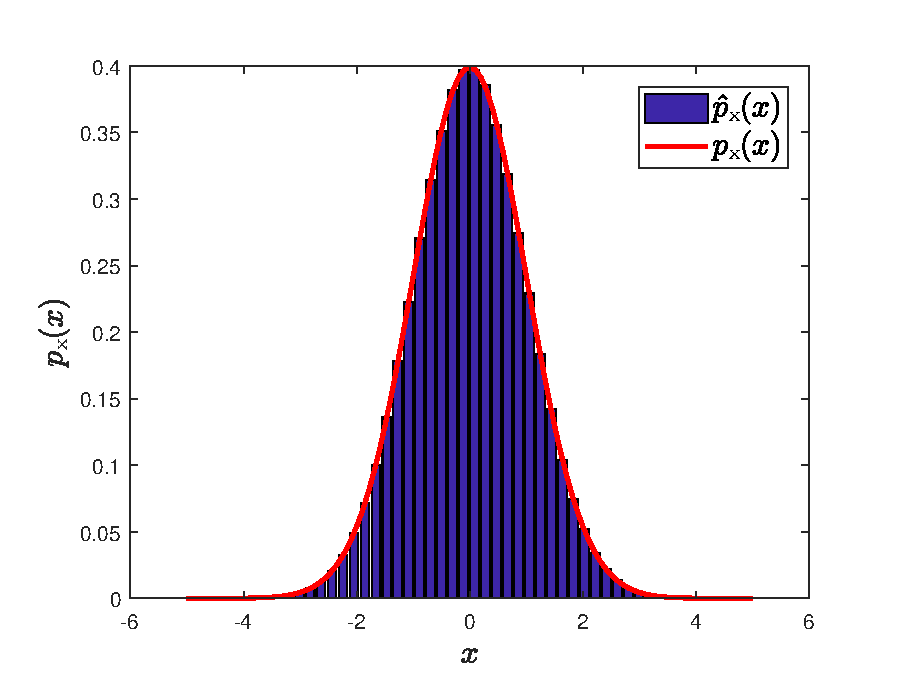
\includegraphics[width = 0.8\textwidth]{pdf_normal.eps}
%       \caption{Gaussian PDF and histogram of samples}
%       \label{fig:1}
%     \end{figure}

%   The source code to plot Figure \ref{fig:1} could be found in Appendix \ref{sec:a:code}. Here are the core codes:
%   \lstinputlisting[firstline=4,lastline=4, firstnumber=4]{matlabscript.m}
%   \lstinputlisting[firstline=6,lastline=7, firstnumber=6]{matlabscript.m}
%   To understand line 6, note that if we have $n$ samples of $X$ denoted by $x^{(i)}, i = 1, 2, \cdots, n$, then the probability density function $p_{X}$ can be estimated as
%   \begin{equation*}
%     \begin{aligned}
%       p_{X}(x_0) &= \left.\frac{\mathrm{d}}{\mathrm{d}x} \Prob(X \leq x) \right|_{x = x_0} \\
%       &\approx \frac{\Prob(x_0 - \Delta x < X \leq x_0)}{\Delta x}\\
%       &\approx \frac{1}{n\Delta x} \sum_{i = 1}^n \1_{x^{(i)} \in (x_0 - \Delta x, x_0]}.
%     \end{aligned}    
%   \end{equation*}
    

  
%   \newpage
  
%   \appendix
%   \section{Source code}
%   \label{sec:a:code}
%   % \lstlistoflistings
%   The source code for plotting Figure \ref{fig:1} is shown as follows.
%   \lstinputlisting{matlabscript.m}
  
\end{document}
%%% Local Variables:
%%% mode: latex
%%% TeX-master: t
%%% End:
